\documentclass[8pt]{beamer}
%epackage[french]{babel}
\usepackage[latin1]{inputenc}
\usepackage{times}
\usepackage{wasysym}
\usepackage[T1]{fontenc}
\usepackage{verbatim}


\definecolor{mongris}{gray}{0.8}           % definition couleur grise
\newcommand{\dd}{\footnotesize $\Diamond$}

\newcommand{\HH}{ \vspace{0.5pt}\hrule}
\newcommand{\round}[1]{\lceil #1 \rfloor}  % notation arrondi
\def\eme{$^{\textrm{{\`e}me}}$}                  % i {\`e}me
\def\num{n^{\circ}}                        % numero
\def\Num{N^{\circ}}                        % Numero
\def\sinc{\mathrm{sinc}}                   % sinus cardinal
\def\ere{$^{\textrm{{\`e}re}}$}                % {\`e}re
\def\er{$^{\textrm{{e}r}}$}                % {\`e}re
\def\eg{\emph{e.g.} }                      % e.g.
\def\ie{\emph{i.e.} }                      % i.e.
\def\etc{\emph{etc.}}                       % etc
\def\cm{\,cm}                              % cm
\def\met{\,m}                              % m
\def\mm{\,mm}                              % mm
\def\deg{$^\circ$}                         % degres
\def\ud{\mathrm{d}}                        % pour dx dy ...


\def \R {{\Bbb R}}
\def \I {{\Bbb I}}
\def \H{{\Bbb H}}
\def \F {{\Bbb F}}
\def \S {{\Bbb S}}
\def \B {{\Bbb B}}
\def \Z {{\mathbb Z}}
\def \G {{\mathbb G}}
\def \L {{\mathcal{L}}}
\def \C {{\mathcal C}}
\def \P {{\mathcal P}}
\def \Q {{\mathcal Q}} 
\def \E{{\mathcal E}}
\def \D{{\mathcal D}}
\definecolor{mybluecolor}{RGB}{116,121,149}

\newcommand{\darky}[1]{{\usebeamercolor[fg]{block title example} #1}}
\newcommand{\myblue}[1]{{\color{mybluecolor}\aut{[#1]}}}

\newcommand{\ball}  {\ensuremath{B}}
\newcommand{\AMDR}{\operatorname{AMD}}
\newcommand{\AMD}{\operatorname{AMD}}

\newcommand{\MAset}{\ensuremath{\mathrm{A\!M}} }
\newcommand{\MAsetg}{\ensuremath{\MAset^g } }

\def \PS {{\aut{Planar-4-3-SAT}}}
\def \R {{\Bbb R}}
\def \I {{\Bbb I}}
\def \F {{\Bbb F}}
\def \S {{\Bbb S}}
\def \Z {{\mathbb Z}}
\def \L {{\mathcal{L}}}
\def \C {{\mathcal C}}
\def \P {{\mathcal P}}
\def \Q {{\mathcal Q}} 
\def \E{{\mathcal E}}
\def \D{{\mathcal D}}
\def \BD {{\bar{\mathcal{D}}}}
\def \etal {{\it et al.~}}
\def\arc{\mbox{arc}}
\definecolor{mongris}{gray}{0.8}          
\newcommand{\fup}[1]{\uparrow#1\uparrow}
\newcommand{\fdown}[1]{\downarrow#1\downarrow}
\newcommand{\sI}[1]{\overline{\tt #1}}
\newcommand{\iI}[1]{\underline{\tt #1}}
\newcommand{\e}[5]{#1 & #2 & #3 & #4 & #5 \\}
\newcommand{\eh}[5]{\text{#1} & \text{#2} &  \text{#3} &  \text{#4} & \text{#5}\\} 

\usepackage{beamerthemeliris2}
\useoutertheme{smoothbars}

\title[DGtal]{DGtal: Digital  Geometry Tools and Algorithms Library}
\subtitle{1D Geometry}

%\author{}
\author[~~~~~~~~~~~~~~~~~~~~~~~~~~~~~~~Tristan Roussillon]{Tristan Roussillon}


 \newcommand{\fod}[2]{\multicolumn{2}{p{3.5cm}}{\emph{#1}\dotfill} &
      \multicolumn{2}{p{9cm}}{#2}\\}
    \newcommand{\fodt}[4]{\emph{#1} & {\footnotesize \textsl{#2}} & #3 & \small #4\\}
    % \newenvironment{ta}{\begin{tabular}{p{3.5cm}p{9cm}}}{\end{tabular}\\}
    \newenvironment{ta}{\begin{tabular}{crll}}{\end{tabular}\\}
    % \vfill


\newcommand{\aut}[1]{{\sc #1}}             % auteur en small capsu


%\institute%[XXX]
%{%
%
%  {\bf Laboratoire d'InfoRmatique en Image et Syst�mes d'information} \\
%  { \scriptsize{
%  LIRIS UMR 5205 CNRS/INSA de Lyon/Universit� Claude Bernard Lyon 1/Universit� Lumi�%re Lyon 2/Ecole Centrale de Lyon\\
%  INSA de Lyon, b�timent J. Verne\\
%  20, Avenue Albert Einstein - 69622 Villeurbanne cedex\\
%  \url{http://liris.cnrs.fr}}
%  }
%}



\graphicspath{{./Images/}}


\begin{document}

\small








\begin{frame}[plain]
  \titlepage
\end{frame}



%\begin{frame}
%  \frametitle{Table of Contents}
%  \tableofcontents
%\end{frame}

\begin{frame}
\frametitle{Objectives}

Tools that help in analysing any one-dimensional discrete structures in a generic framework. 

  \begin{block}{Examples in digital geometry}
    \begin{itemize}
    \item digital curves
      \begin{itemize}
      \item 2d, 3d, nd
      \item 4-connected, 8-connected, disconnected
      \item pixels, interpixels, points
      \item open or closed
      \end{itemize}
		\item chain codes
    \end{itemize}
  \end{block}

\alert{Constant structures, not mutable} 

\end{frame}

\section{Iterators/Circulators and Ranges}


\begin{frame}
  \frametitle{Structures}

  \begin{block}{2 characteristics}
    \begin{itemize}
		\item discrete
    \item one-dimensional
    \end{itemize}
  \end{block}

  \begin{block}{2 notions}
    \begin{itemize}
    \item element
    \item local order (next and previous element)
    \end{itemize}
  \end{block}



\end{frame}

\begin{frame}
  \frametitle{Iterators}

  \begin{block}{Iterator}
    \begin{itemize}
    \item operator* (to get the element)
    \item operator++, operator- - (to point to the next and previous element)
    \end{itemize}
  \end{block}

  \begin{block}{Reachability}
An iterator j is reachable from an iterator i if and only if i can be made equal to j with finitely many applications of the operator++. 
  \end{block}

  \begin{block}{Range}
If j is reachable from i, one can iterate over the range of elements bounded by i and j, from the one pointed to by i and up to but not including the one pointed to by j. Such a range is valid and is denoted by [i,j).
  \end{block}

\end{frame}

\begin{frame}
  \frametitle{Open/Linear structures}

  \begin{block}{Classic iterator}
\begin{itemize}
  \item past-the-end value
  \item $[begin,end)$ is the whole range
  \item $[i,j)$ is not always valid
  \item $[i,i)$ is the empty range
\end{itemize}
  \end{block}

%image
 \begin{center}
   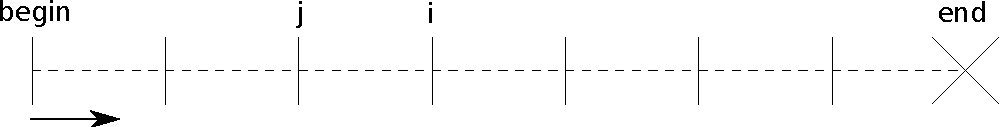
\includegraphics[width=1\textwidth]{linearRange}
 \end{center}

\end{frame}

\begin{frame}
  \frametitle{Closed/Circular structures}

  \begin{block}{CGAL circular iterator (circulator)}
\begin{itemize}
  \item no past-the-end value
  \item $[i,j)$ is always valid
  \item $[i,i)$ is the whole range
  \item As long as $i \neq j$, the range $[i,j)$ behaves like a classic iterator range. 
\end{itemize}
  \end{block}

%image
 \begin{center}
   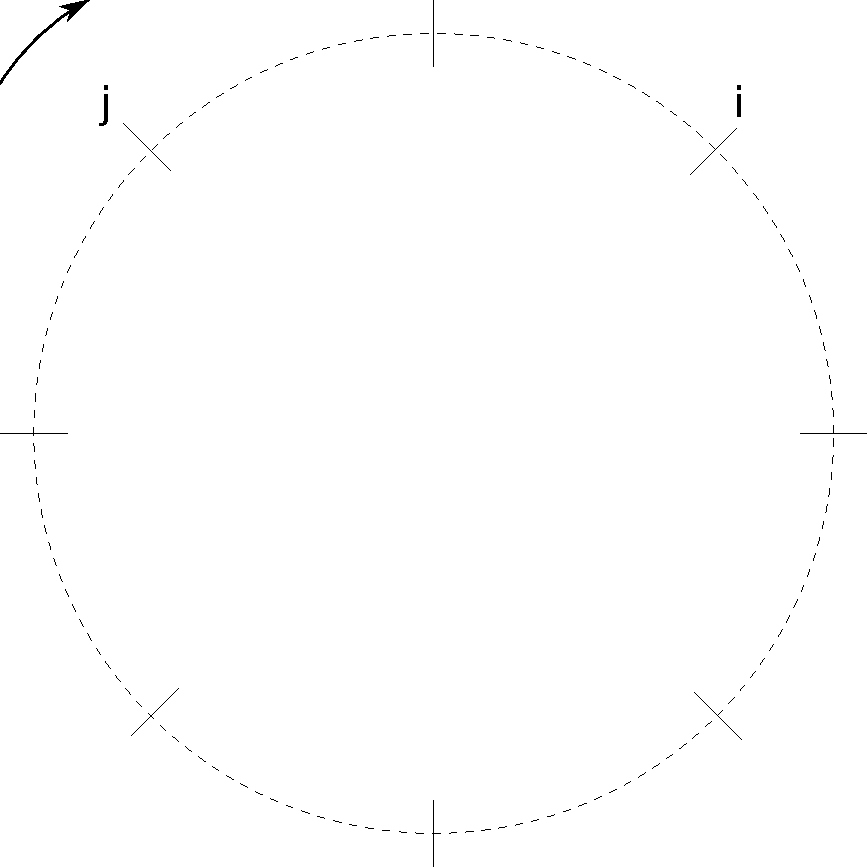
\includegraphics[width=0.6\textwidth]{circularRange}
 \end{center}

\end{frame}

\begin{frame}
  \frametitle{Scanning backward}

  \begin{block}{Reverse iterator}
A reverse iterator is an adaptor for scanning backward. The operator++ of the adaptor calls the operator-- of the underlying (circular)iterator and conversely. You can use the STL reverse iterator.
  \end{block}

  \begin{block}{Tricky part}
Operator* of the adaptor calls operator- - of the underlying (circular)iterator before calling its operator*.
  \end{block}

%image
 \begin{center}
   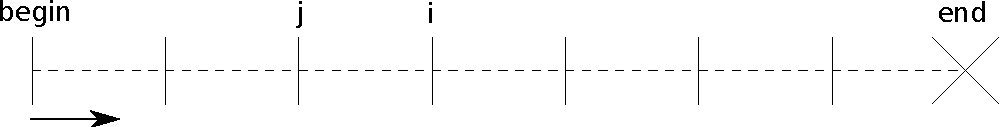
\includegraphics[width=1\textwidth]{linearRange}
 \end{center}

\end{frame}


\section{Classes}

\begin{frame}
  \frametitle{GridCurve}

  \begin{block}{}
GridCurve is an (open or closed) n-dimensional oriented grid curve. It stores a list of alternated (signed) 0-cells and 1-cells. 
  \end{block}

%image
 \begin{center}
   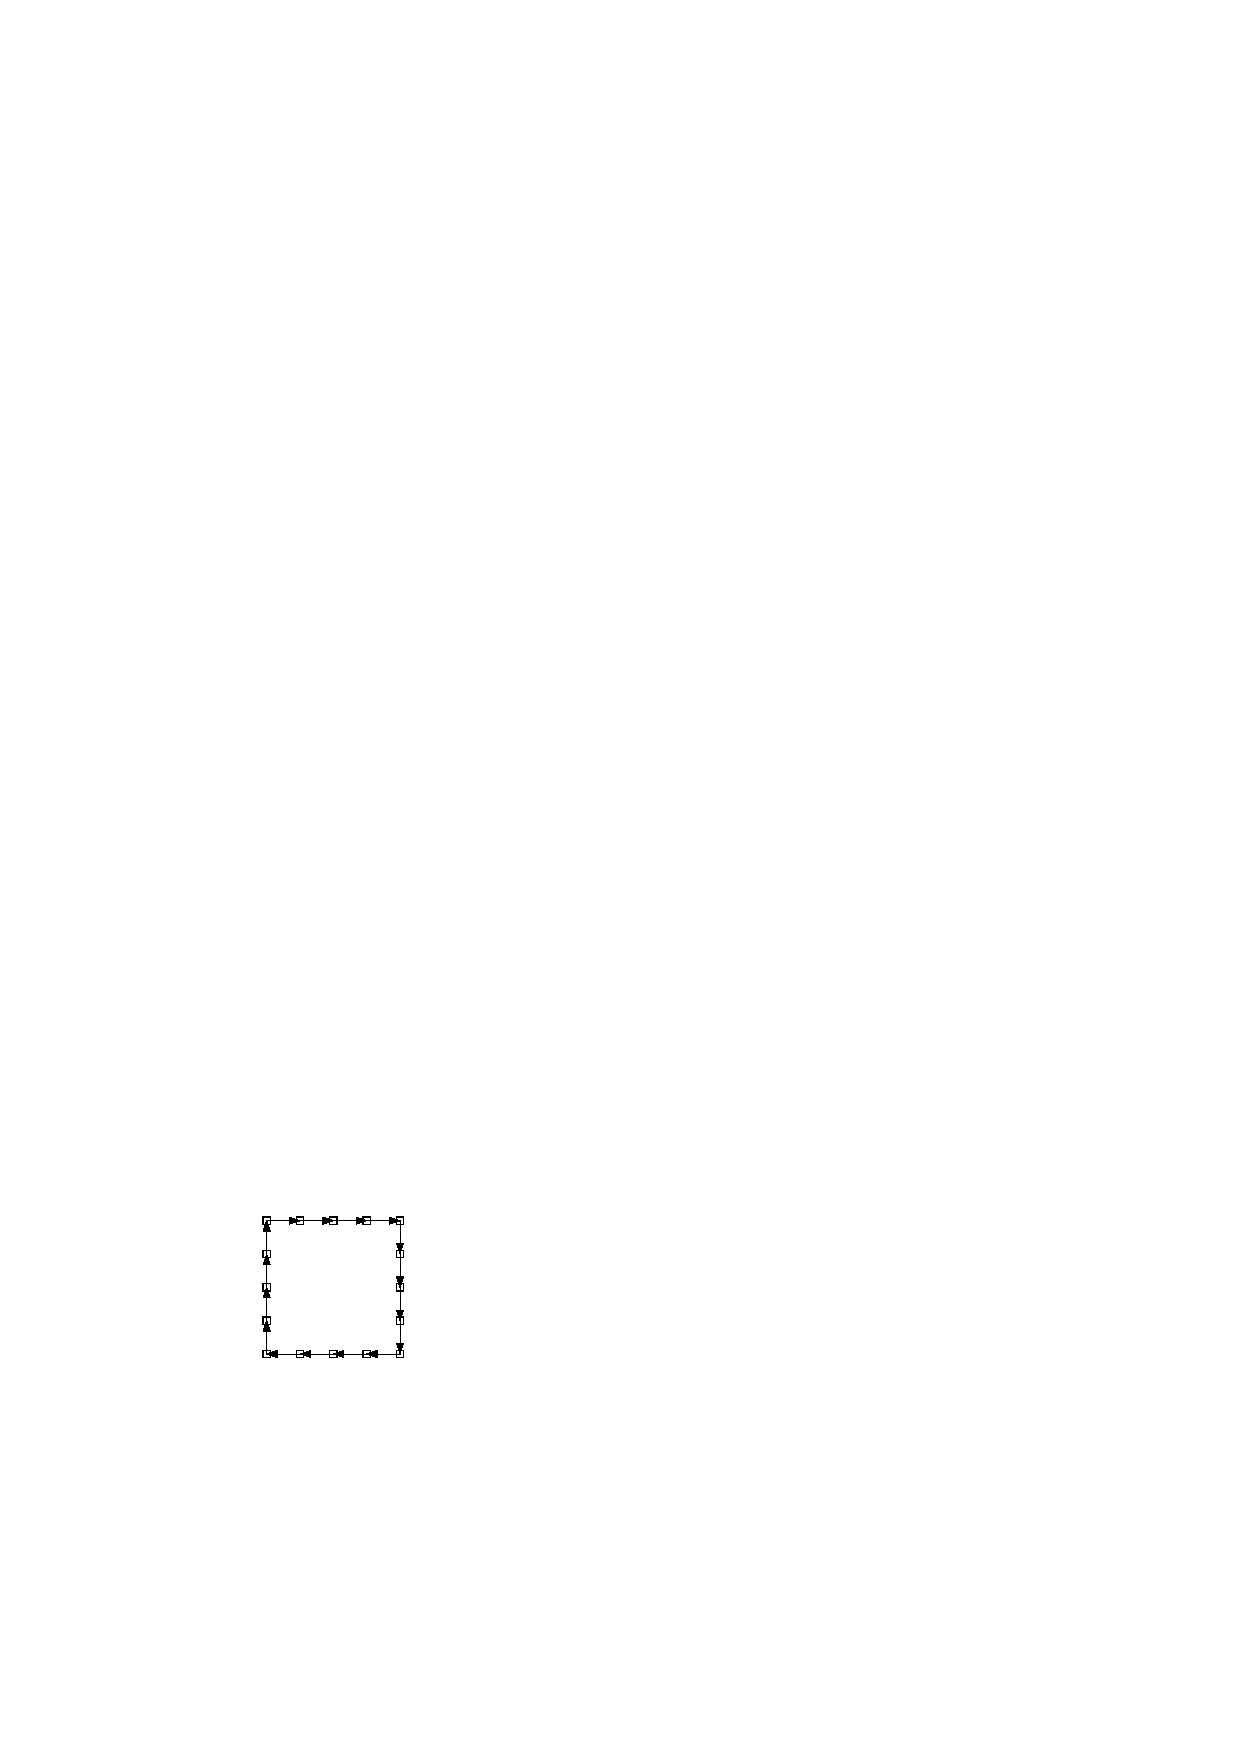
\includegraphics[width=0.5\textwidth,page=1]{gridcurve}
 \end{center}

\end{frame}

\begin{frame}
  \frametitle{GridCurve}

  \begin{block}{Ranges}
GridCurve provides many ranges as nested types to iterate over different kinds of elements:
\begin{itemize}
 \item nd
  \begin{itemize}
   \item<1-2> SCellsRange
   \item<3> PointsRange
   \item<4> MidPointsRange
   \item<5> ArrowsRange
  \end{itemize}
 \item 2d TODO
  \begin{itemize}
   \item<6> InnerPointsRange
   \item<7> OuterPointsRange
   \item<8> IncidentPointsRange
   \item CodesRange
  \end{itemize}
\end{itemize}
  \end{block}

\only<1>{
 \begin{center}
   \includegraphics[width=0.25\textwidth,page=2]{gridcurve}
 \end{center}
}
\only<2>{
 \begin{center}
   \includegraphics[width=0.25\textwidth,page=3]{gridcurve}
 \end{center}
}
\only<3>{
 \begin{center}
   \includegraphics[width=0.25\textwidth,page=5]{gridcurve}
 \end{center}
}
\only<4>{
 \begin{center}
   \includegraphics[width=0.25\textwidth,page=4]{gridcurve}
 \end{center}
}
\only<5>{
 \begin{center}
   \includegraphics[width=0.25\textwidth,page=6]{gridcurve}
 \end{center}
}
\only<6>{
 \begin{center}
   \includegraphics[width=0.25\textwidth,page=7]{gridcurve}
 \end{center}
}
\only<7>{
 \begin{center}
   \includegraphics[width=0.25\textwidth,page=8]{gridcurve}
 \end{center}
}
\only<8>{
 \begin{center}
   \includegraphics[width=0.25\textwidth,page=9]{gridcurve}
 \end{center}
}
\end{frame}

\begin{frame}
  \frametitle{Code}

  \begin{block}{FreemanChain}
FreemanChain is 2-dimensional and 4-connected digital curve stored as a string of codes {0,1,2,3}. 
As GridCurve, it provides a CodesRange.
  \end{block}

  \begin{block}{Conversion between FreemanChain and GridCurve}
TODO
  \end{block}

\end{frame}








\section{Segments and segment computers}

  \begin{frame}<beamer>
    \frametitle{Plan}
    \tableofcontents[sectionstyle=show/shaded]
  \end{frame}

\begin{frame}
  \frametitle{Segments}
 

   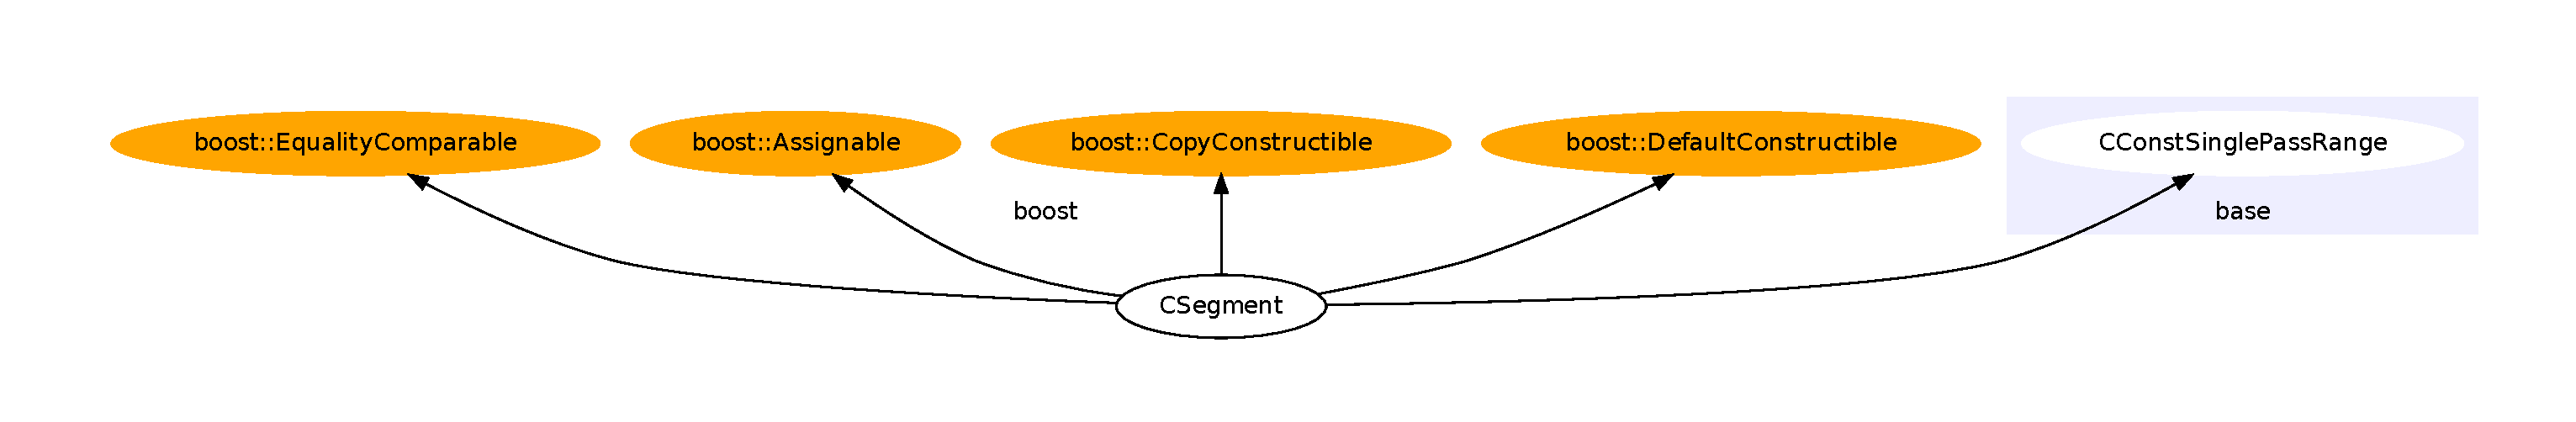
\includegraphics[width=1\textwidth]{segmentGraph}

  \begin{block}{Segment}
It is a valid and \emph{not empty} range. 

~

Type:
\begin{itemize}
  \item ConstIterator: at least a model of a \emph{bidirectional} iterator
\end{itemize}

Main methods:
\begin{itemize}
  \item begin(): begin iterator of the range
  \item end(): end iterator of the range (past-the-end)
\end{itemize}

Invariant: ( begin() != end() )
  \end{block}

\end{frame}

\begin{frame}
  \frametitle{The detection problem}
 
  \begin{block}{Class of segments $\Sigma_P$}
Set of segments such that for each segment of the set, 
a given predicate $P$ is true: 

$\forall s \in \Sigma_P,  P(s) = \text{true}$ 
  \end{block}

  \begin{block}{Detection problem}
Deciding whether a given segment 
belongs to a class of segments or not:  

is $s \in \Sigma_P$ ? or equivalently is $P(s)$ true ? 
  \end{block}

  \begin{block}{Segment computer}
Segment that can 
\begin{enumerate}
 \item constructs other instances of its own type
 \item control its own extension so that the predicate $P$ remains true
\end{enumerate}
  \end{block}

\end{frame}

\begin{frame}
  \frametitle{Segment computers}
 

 \begin{center}
   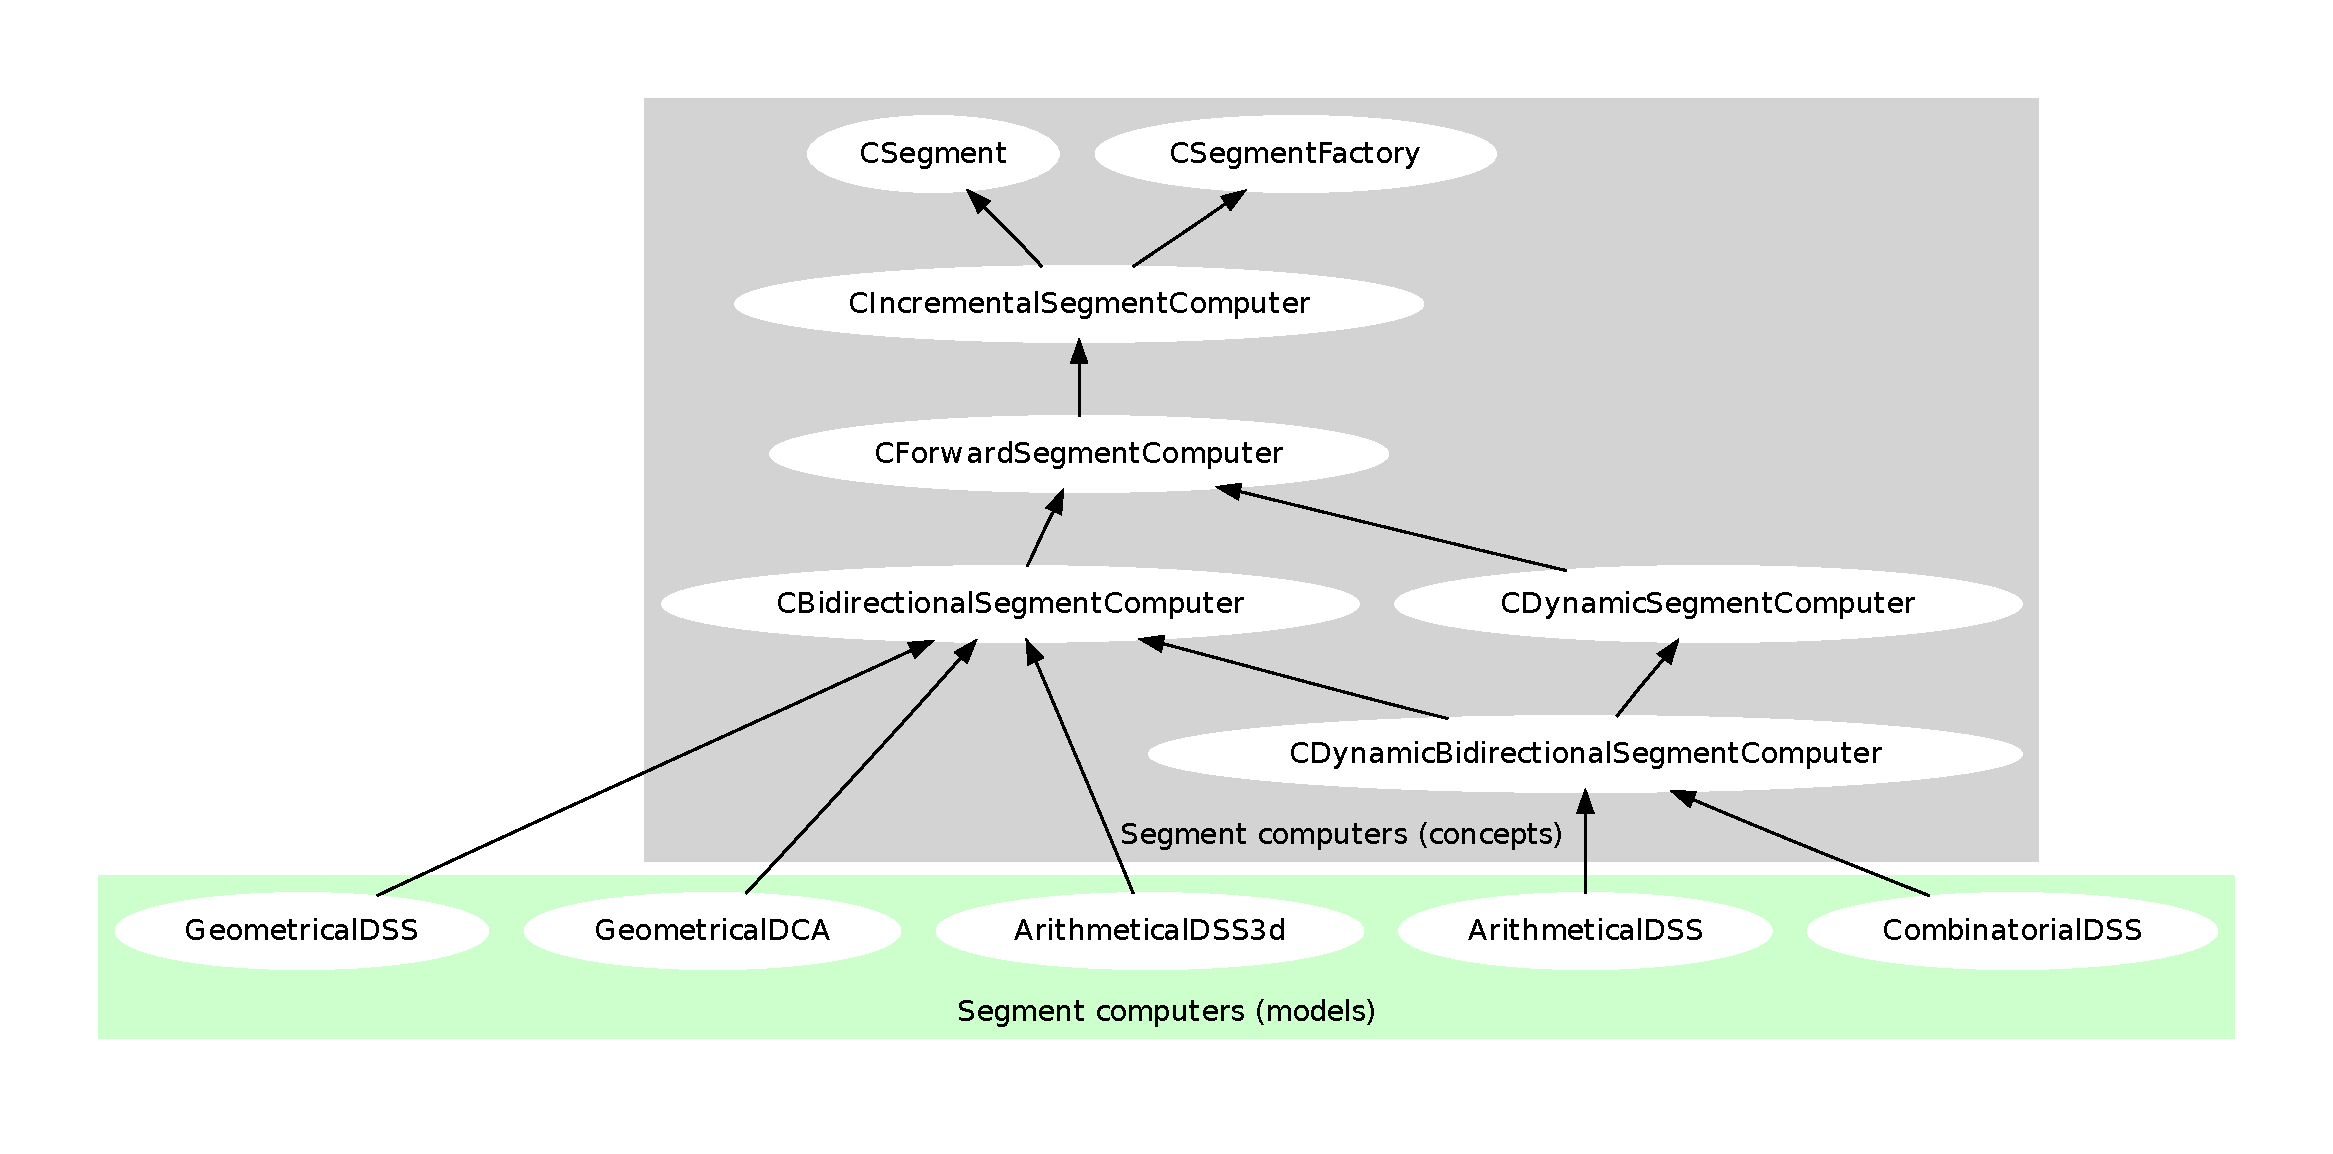
\includegraphics[width=1\textwidth]{segmentComputersGraph}
 \end{center}

\end{frame}

\begin{frame}[containsverbatim,fragile]
  \frametitle{CIncrementalSegmentComputer: syntactic constraints}

Refinement of CSegment and CSegmentFactory that provides in addition the following methods:
\begin{itemize}
 \item void init ( const ConstIterator\& it ) : set the segment to the element pointed by it.
 \item bool isExtendable () : return 'true' if the segment can be extended to the element pointed by end() and 'false' otherwise (no extension is performed).
 \item bool extend () : return 'true' and extend the segment to the element pointed by end() if it is possible, return 'false' and does not extend the segment otherwise.
\end{itemize}

~

Detection of a segment:
  \begin{lstlisting}
    //s is a segment computer
    //[begin,end) is a range
    s.init( begin );
    while ( (s.end() != end) && (s.extend()) ) {} 
  \end{lstlisting}

Avoiding infinite loops with circulators:
  \begin{lstlisting}
    //s is a segment computer
    //c is a circulator
    s.init( c );
    while ( (s.end() != s.begin()) && (s.extend()) ) {}
  \end{lstlisting}

\end{frame}

%incremtal vs forward
\begin{frame}[containsverbatim,fragile]
  \frametitle{CIncrementalSegmentComputer vs CForwardSegmentComputer}

Same syntactic constraints but different semantic constraints

~

Models of CIncrementalSegmentComputer verify: 
  \begin{lstlisting}
for ( ConstIterator it = s.begin(), 
      ConstIterator itEnd = s.end();
      it != itEnd; ++it)
  { // [s.begin(), it) is a segment:
    s.init( s.begin() ); 
    bool flag = true; 
    while ( (s.end() != it)&&(flag) ) { flag = s.extend(); }
    ASSERT( flag ); 
  }
  \end{lstlisting}

In addition, models of CForwardSegmentComputer verify: 
  \begin{lstlisting}
for ( ConstIterator it = s.begin(), 
      ConstIterator itEnd = s.end();
      it != itEnd; ++it)
  { // [it, itEnd) is a segment:
    bool flag = true; 
    while ( (s.end() != itEnd)&&(flag) ) { flag = s.extend(); }
    ASSERT( flag ); 
  }
  \end{lstlisting}

\end{frame}

\begin{frame}
  \frametitle{Useful functions}
 
The code can be different if an iterator or a circulator is used as the nested ConstIterator type. Moreover, some tasks can be made faster for a given kind of segment computer than for another kind of segment computer. Basically, 
given a maximal segment, computing the next maximal segment is faster for dynamic segment computers than for forward segment computers. That's why many generic functions are provided in SegmentComputerUtils.h:

\begin{itemize}
 \item maximalExtension, oppositeEndMaximalExtension, maximalSymmetricExtension,
 \item maximalRetraction, oppositeEndMaximalRetraction,
 \item longestSegment (init the segment computer),
 \item firstMaximalSegment, lastMaximalSegment, mostCenteredMaximalSegment,
 \item previousMaximalSegment, nextMaximalSegment,
\end{itemize}



\end{frame}






\section{Segmentations}

\begin{frame}
  \frametitle{Segmentations}
 
  \begin{block}{Definition}
A segmentation is an \emph{ordered} set of segments (of a same class) \emph{spanning} a given range. 

~

A given range contains a finite set of segments of a given class. 
A segmentation is a subset of the whole set of segments such that:
\begin{enumerate}
 \item (spanning) each element of the range belongs to a segment of the subset
 \item (ordered) no segment contains another segment of the subset 
\end{enumerate}
Due to (2), the segments of a segmentation can be ordered without ambiguity 
(according to the relative position of their first element for instance).
  \end{block}

%  \begin{block}{Main type}
%SegmentComputerIterator
% \begin{itemize}
%  \item dereference operator: return an instance of a segment computer.
%  \item intersectPrevious(), intersectNext(): return 'true' if the current segment intersects, respectively, the %previous and the next one (when they exist), 'false' otherwise.
% \end{itemize}
%  \end{block}

 % \begin{block}{Main method}
%init method taking as input parameters: 
%\begin{itemize}
% \item begin/end (circular)iterators of the range to be segmented
% \item an instance of segment computer
%\end{itemize}
%  \end{block}

 \begin{center}
   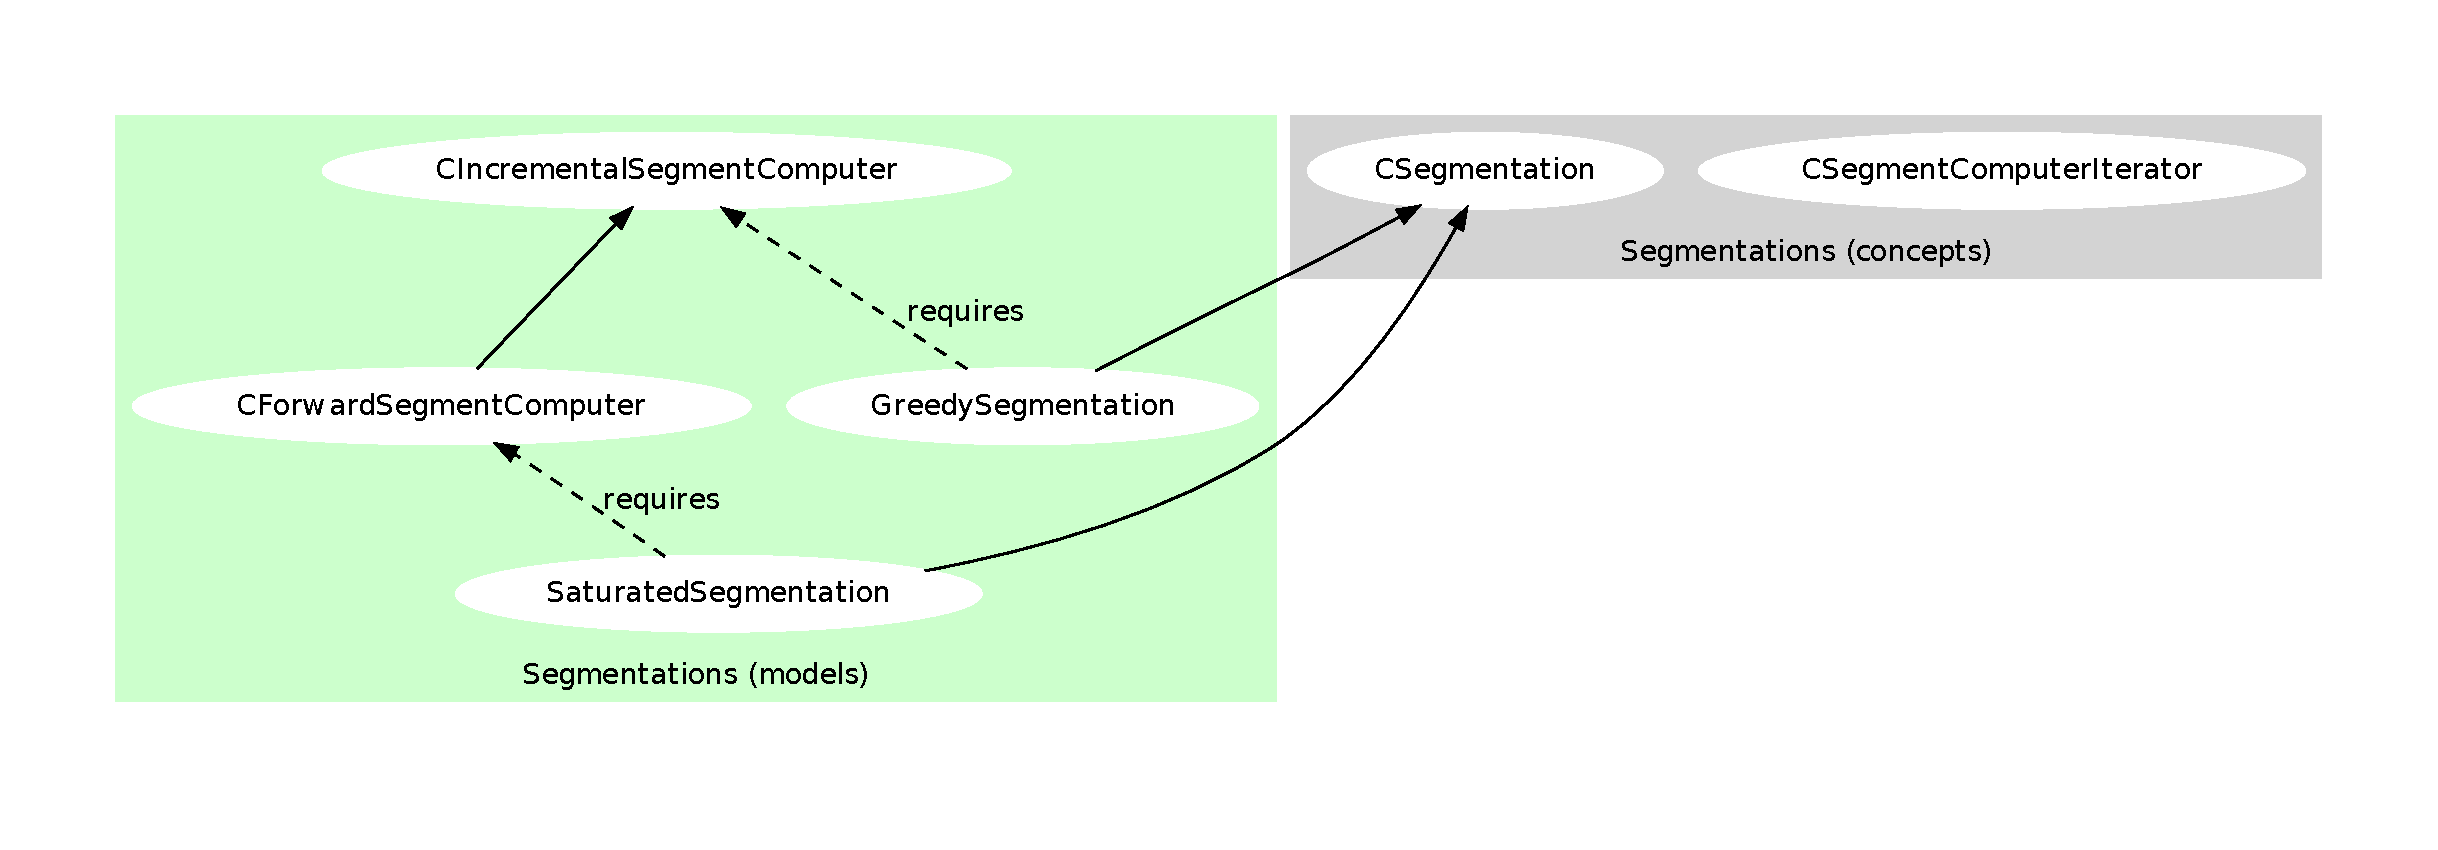
\includegraphics[width=1\textwidth]{segmentationsGraph}
 \end{center}

\end{frame}


\begin{frame}[containsverbatim]
  \frametitle{Example: greedy segmentation into DSS}

  \begin{lstlisting}
  ... // Let r be a range of type Range;

  //types
  typedef ArithmeticalDSS<Range::ConstIterator> SegmentComputer;
  typedef GreedySegmentation<SegmentComputer> Segmentation;

  //instances
  SegmentComputer detectionAlgorithm;
  Segmentation theSegmentation(r.begin(), r.end(), detectionAlgorithm);
                                 
  typedef Segmentation::SegmentComputerIterator SCIterator;  
  SCIterator it = theSegmentation.begin();
  SCIterator itEnd = theSegmentation.end();
  for ( ; it != itEnd; ++it) 
    {
     SegmentComputer current(*it);
     ...
    }
  \end{lstlisting}

 \begin{center}
   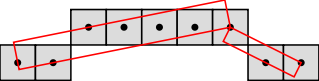
\includegraphics[width=0.45\textwidth]{left_right}
 \end{center}

\end{frame}


\begin{frame}[containsverbatim]
  \frametitle{Other segmentations}

  \begin{lstlisting}
...
  typedef ArithmeticalDSS<Range::ConstReverseIterator> SegmentComputer;
...
  Segmentation theSegmentation(r.rbegin(), r.rend(), detectionAlgorithm);
...
  \end{lstlisting}

 \begin{center}
   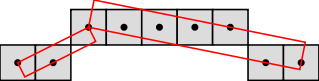
\includegraphics[width=0.45\textwidth]{right_left}
 \end{center}

  \begin{lstlisting}
...
   typedef SaturatedSegmentation<SegmentComputer> Segmentation;
...
  \end{lstlisting}

 \begin{center}
   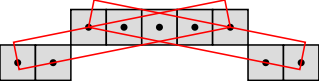
\includegraphics[width=0.45\textwidth]{maxseg}
 \end{center}

\end{frame}

\begin{frame}[fragile]
  \frametitle{Segmentation of subranges}

  \begin{verbatim}
theSegmentation.setSubRange(beginIt, endIt);
theSegmentation.setMode("myMode");
  \end{verbatim}

\begin{itemize}
 \item GreedySegmentation
  \begin{itemize}
   \item \alert<1>{"Truncate" (default)}
   \item "Truncate+1"
   \item "DoNotTruncate"
  \end{itemize}
 \item SaturatedSegmentation
  \begin{itemize}
   \item "First",
   \item \alert<2>{"MostCentered" (default)}
   \item "Last"
  \end{itemize}
\end{itemize}

\only<1>{
\begin{center}
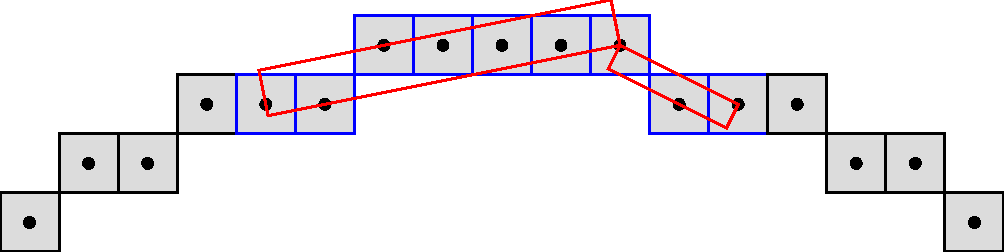
\includegraphics[height=0.2\textheight]{greedyseg-Truncate}
\end{center}
}
\only<2>{
\begin{center}
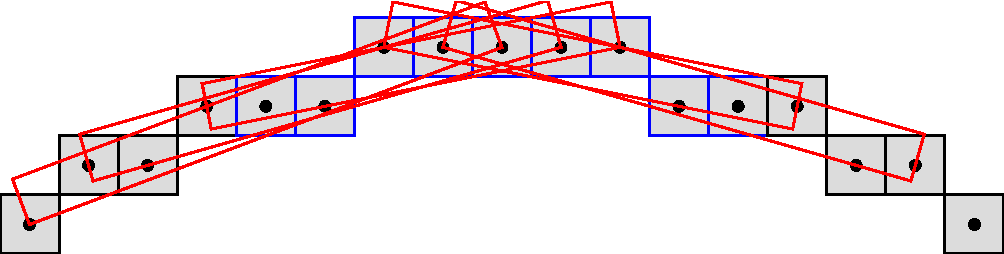
\includegraphics[height=0.2\textheight]{saturatedseg-MostCentered}
\end{center}
}

%NB: a whole range in a closed/circular structure 
%may be viewed as a subrange of a periodic signal. 
\end{frame}

\begin{frame}
  \frametitle{Done (red) and to do (black)}
 

\begin{block}{Segment computers}
\begin{itemize}
  \item \alert{ArithmeticalDSS}
  \item \alert{ArithmeticalDSS3d} (I. Sivignon)
  \item \alert{CombinatorialDSS} (X. Proven\c{c}al)
  \item \alert{GeometricalDSS}
  \item \alert{GeometricalDCA}
  \item ThickSegment
  \item ConvexPart
  \item other based on linear programming
\end{itemize}
\end{block}

\begin{block}{Segmentations}
\begin{itemize}
  \item \alert{GreedySegmentation}: with overlapping at one point (for polygonalisations)
  \item greedy segmentation without overlapping (to get a partition)
  \item greedy segmentation into a minimal number of segments for closed structures 
  \item \alert{SaturatedSegmentation}: all maximal segments
  \item segmentation into a minimal number of \emph{maximal} segments
  \item pencil structure (all segments intersecting at a given element)
\end{itemize}
\end{block}

\end{frame}

\begin{frame}[squeeze]
  \frametitle{Module description (as of 0.5)}

  \begin{block}{Content}
    \begin{itemize}
      \small
    \item One data structure based on a cellular grid space (GridCurve),
    \item which provides different views of the same digital curve (XXXRange).
    \item A segmentation framework (concepts of segment computers and segmentations).
    \item Many detection algorithms (models of segment computers).
    \end{itemize}
  \end{block}

  \begin{block}{Examples}
    \begin{itemize}
      \small
    \item GridCurve (d=1,n=2), (d=1,n=3), (d=2,n=3)
    \item Greedy/Saturated segmentation of (sub)ranges
    \item ArithmeticalDSS(3d)/CombinatorialDSS/GeometricalDSS, GeometricalDCA
    \item convex and concave parts
    \end{itemize}
  \end{block}

  \begin{block}{Location}
    \begin{itemize}
    \item \texttt{\{DGtal\}/src/DGtal/base} (Iterator/Range stuffs)
    \item \texttt{\{DGtal\}/src/DGtal/geometry/curves} (Geometry part) 
    \item \texttt{\{DGtal\}/tests/geometry/curves}
    \item \texttt{\{DGtal\}/examples/geometry/curves}
    \end{itemize}
  \end{block}

\end{frame}



\end{document}



